\smallframetitle

\section{From 08/07/24 to 12/07/24}
\insertsectionframe

\subsection{further advancement on road detection}
\insertsubsectionframe

\begin{frame}{Cities and big cities connection graph}
    \begin{figure}
        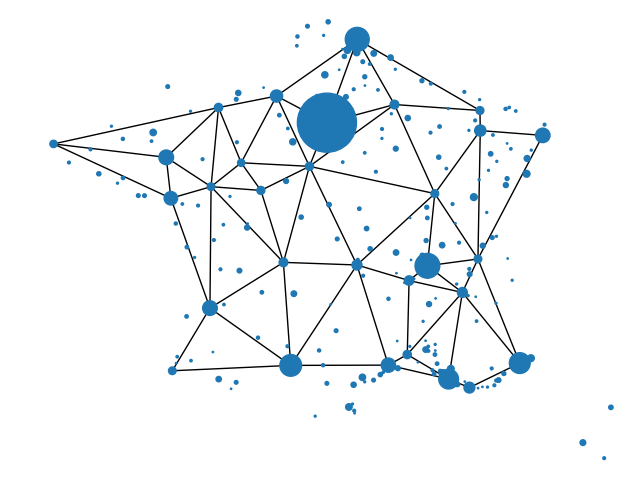
\includegraphics[height=0.6\paperheight]{images/road_detection/city_links_graph_all_cities.png}
        \caption{cities and big cities connection graph}
    \end{figure}
\end{frame}

\begin{frame}{Little cities linking method}
    \begin{block}{Steps}
        \begin{itemize}
            \item For each edge of the connection graph ;
            \item Detect all little cities close enough to this edge ;
            \item Create multiple edges to link all these cities together by a path with the same start and ending city than the big edge ;
        \end{itemize}
    \end{block}
    \begin{columns}
        \begin{column}{0.5\paperwidth}
            \begin{figure}
                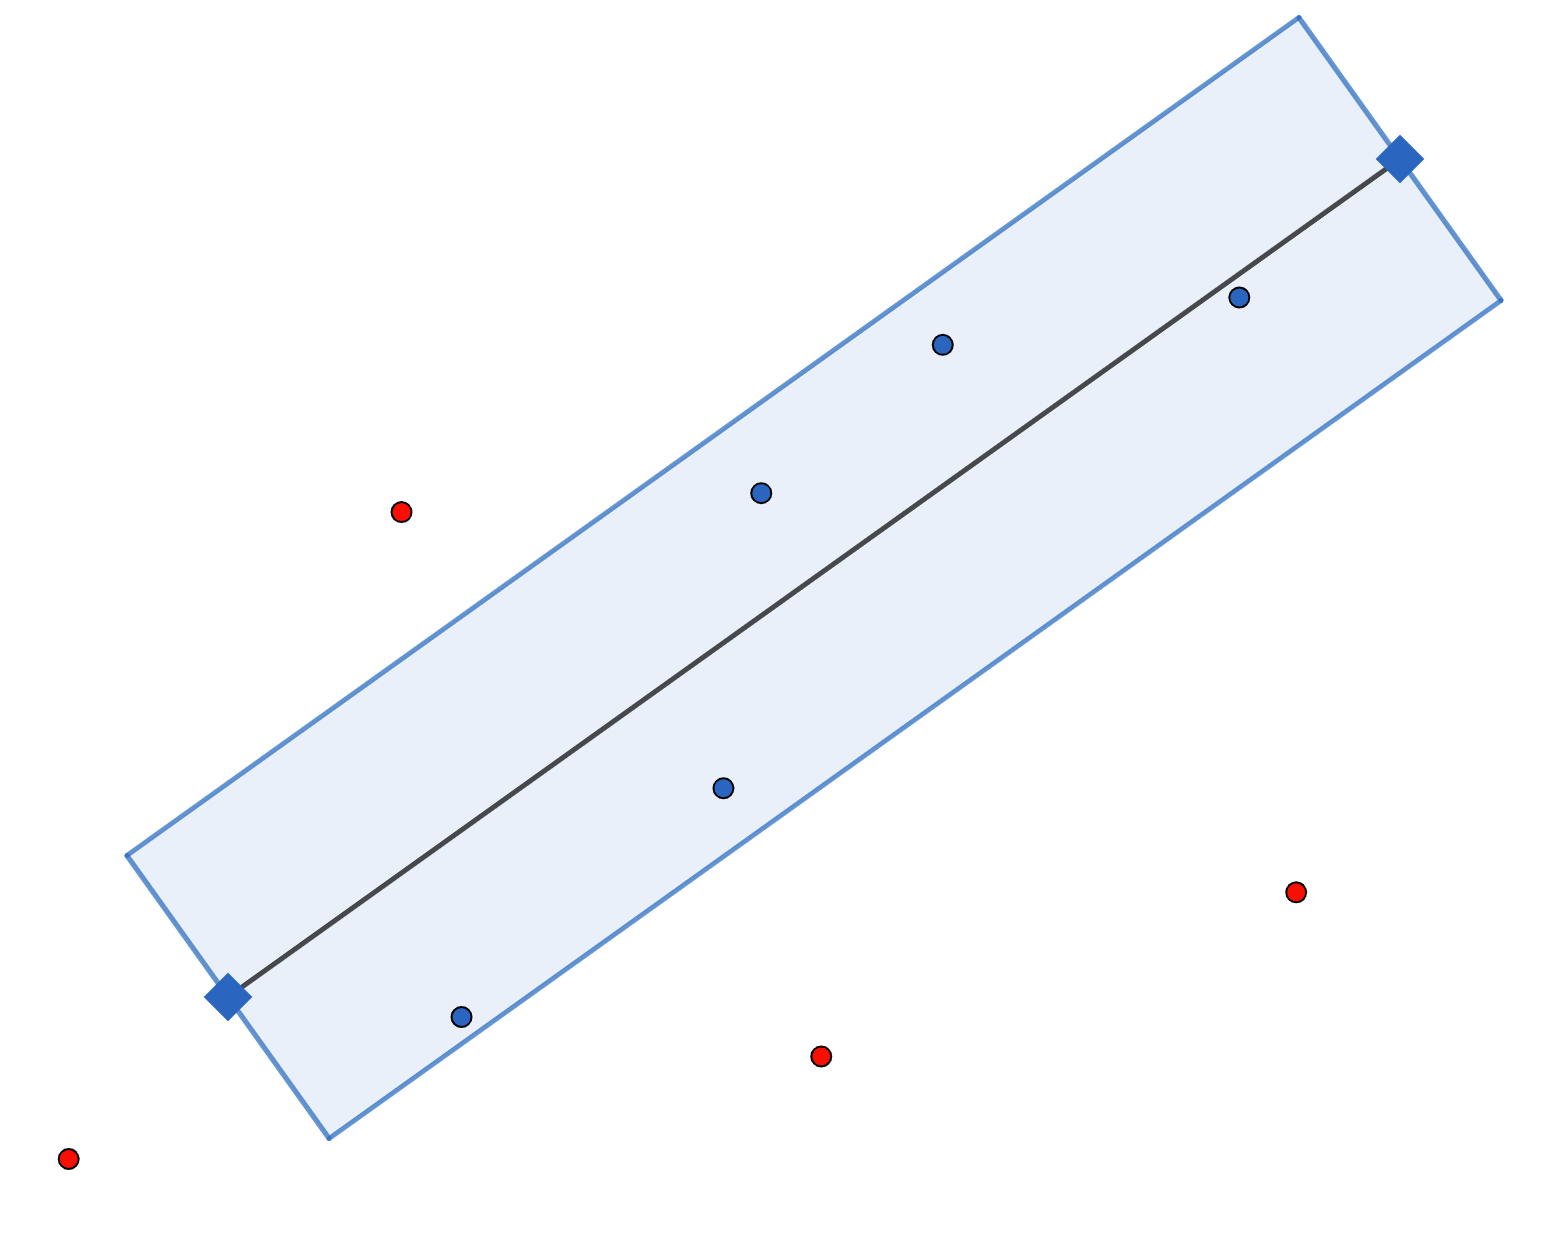
\includegraphics[height=0.3\paperheight]{images/road_detection/illustartion_city_selections.png}
                \caption{Little cities selection}
            \end{figure}
        \end{column}
        
        \begin{column}{0.5\paperwidth}
            \begin{figure}
                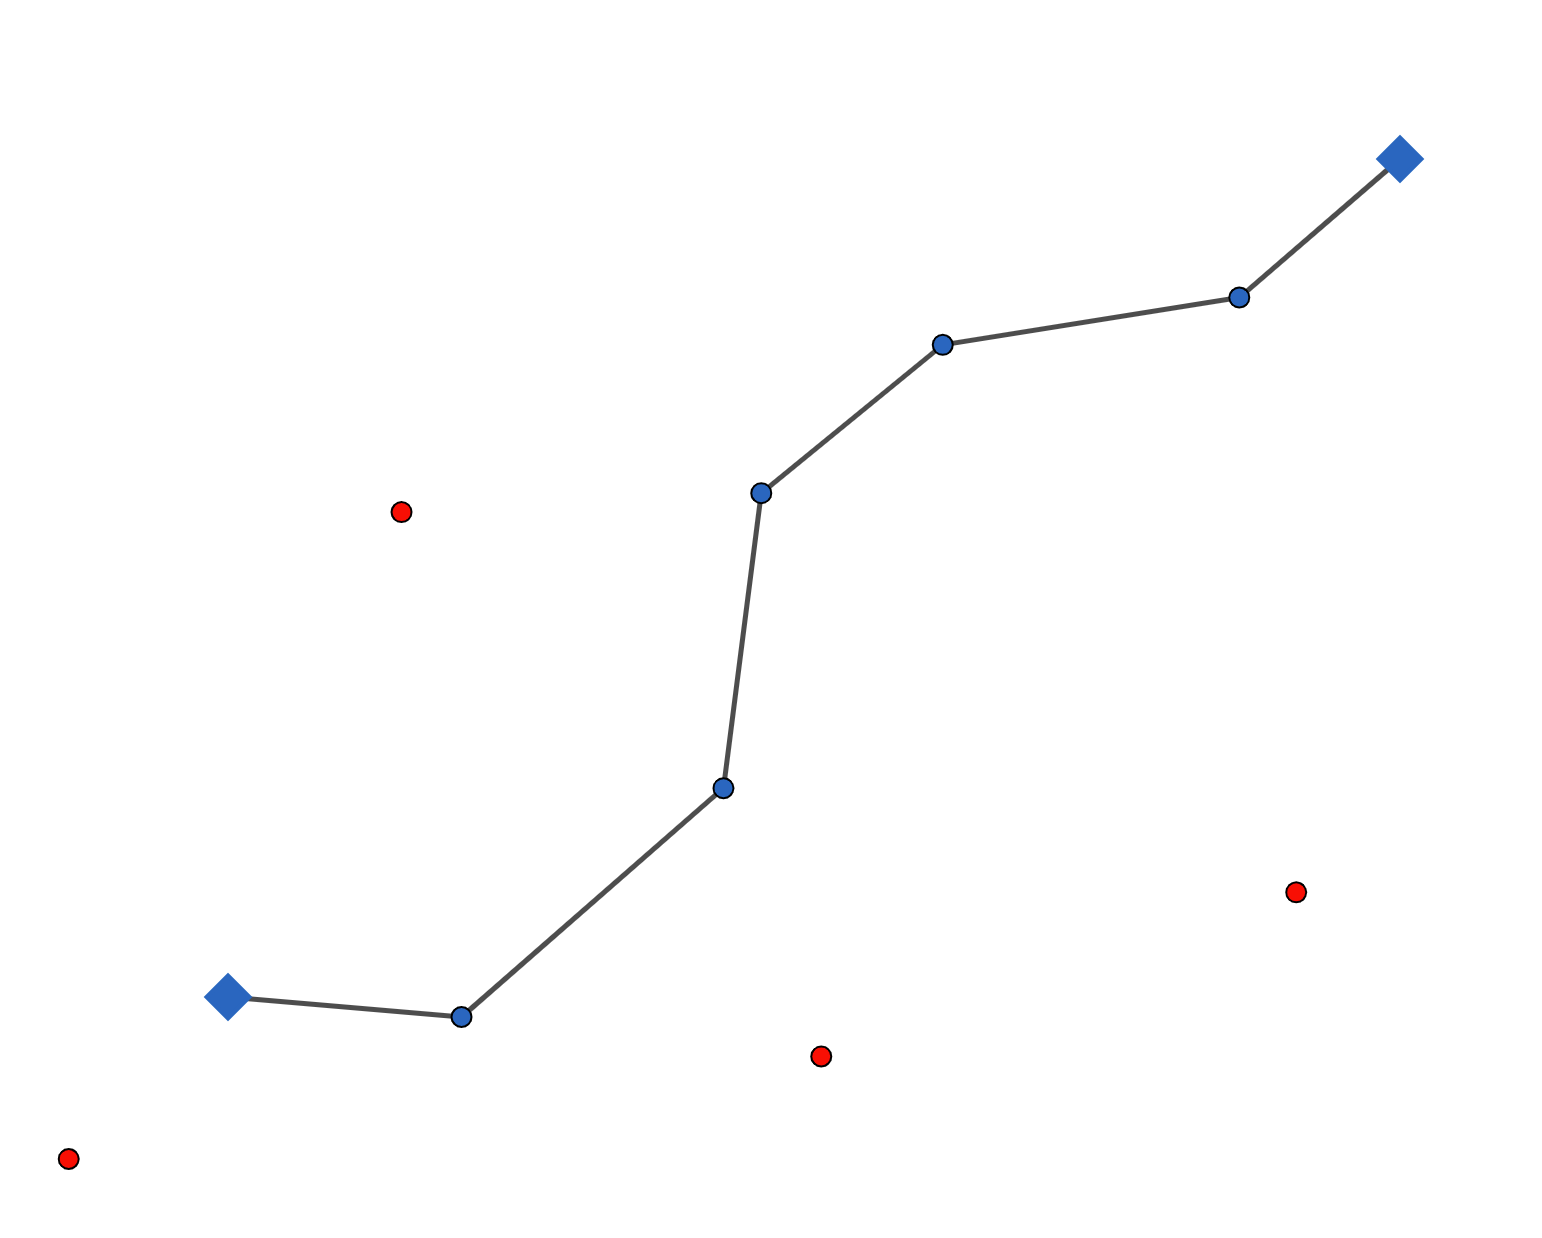
\includegraphics[height=0.3\paperheight]{images/road_detection/illustration_city_linkage.png}
                \caption{Cities linkage}
            \end{figure}
        \end{column}
    \end{columns}
\end{frame}

\begin{frame}{New graph after little city linkage}
    \begin{figure}
        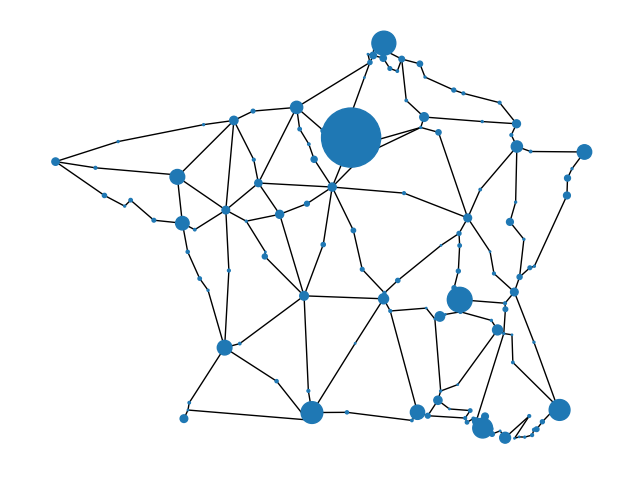
\includegraphics[height=0.6\paperheight]{images/road_detection/final_graph.png}
        \caption{Final graph (width parameter = $0.2$)}
    \end{figure}
\end{frame}

\begin{frame}{New graph on a map}
    \begin{figure}
        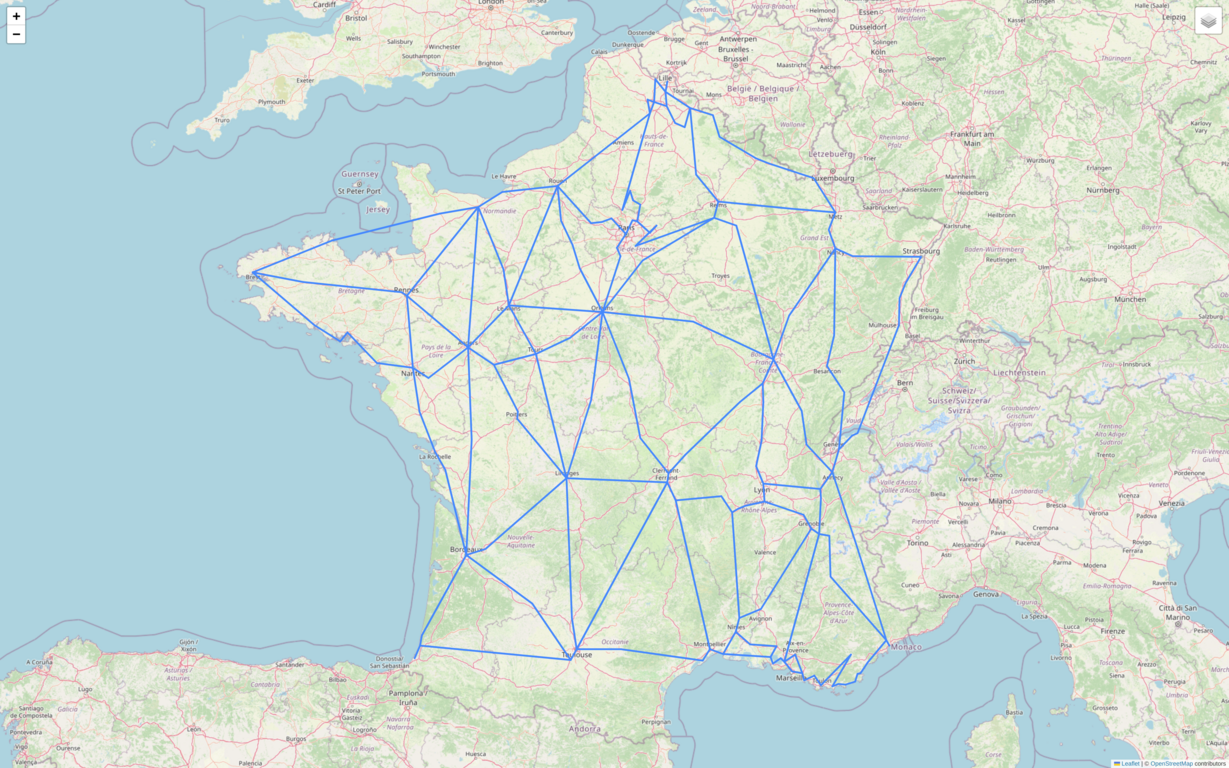
\includegraphics[height=0.6\paperheight]{images/road_detection/final graph on map.png}
        \caption{Final graph on a map (width parameter = $0.2$)}
    \end{figure}
\end{frame}

\begin{frame}{Reminder : pre-road detection thanks to the clustering methods}
    \begin{figure}
        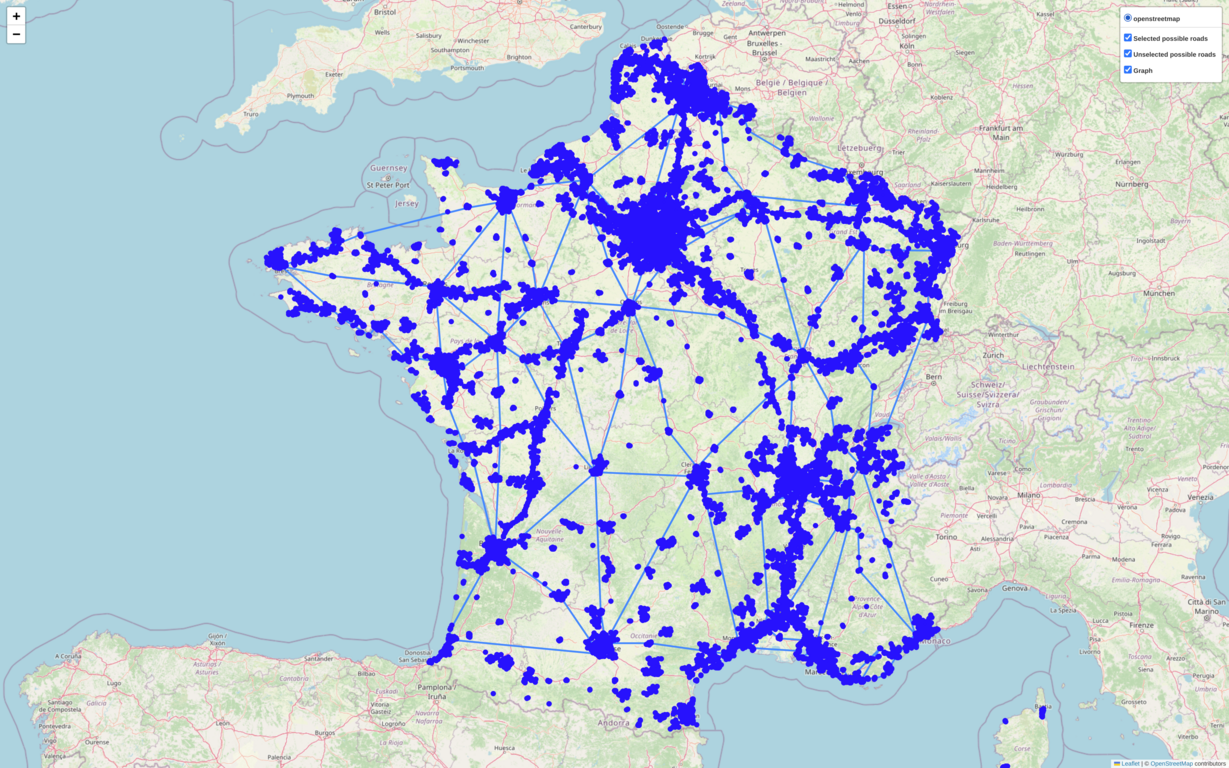
\includegraphics[height=0.6\paperheight]{images/road_detection/road-predetection and graph.png}
        \caption{Road pre-detection and graph}
    \end{figure}
\end{frame}

\begin{frame}{Final selected road base stations}
    \begin{figure}
        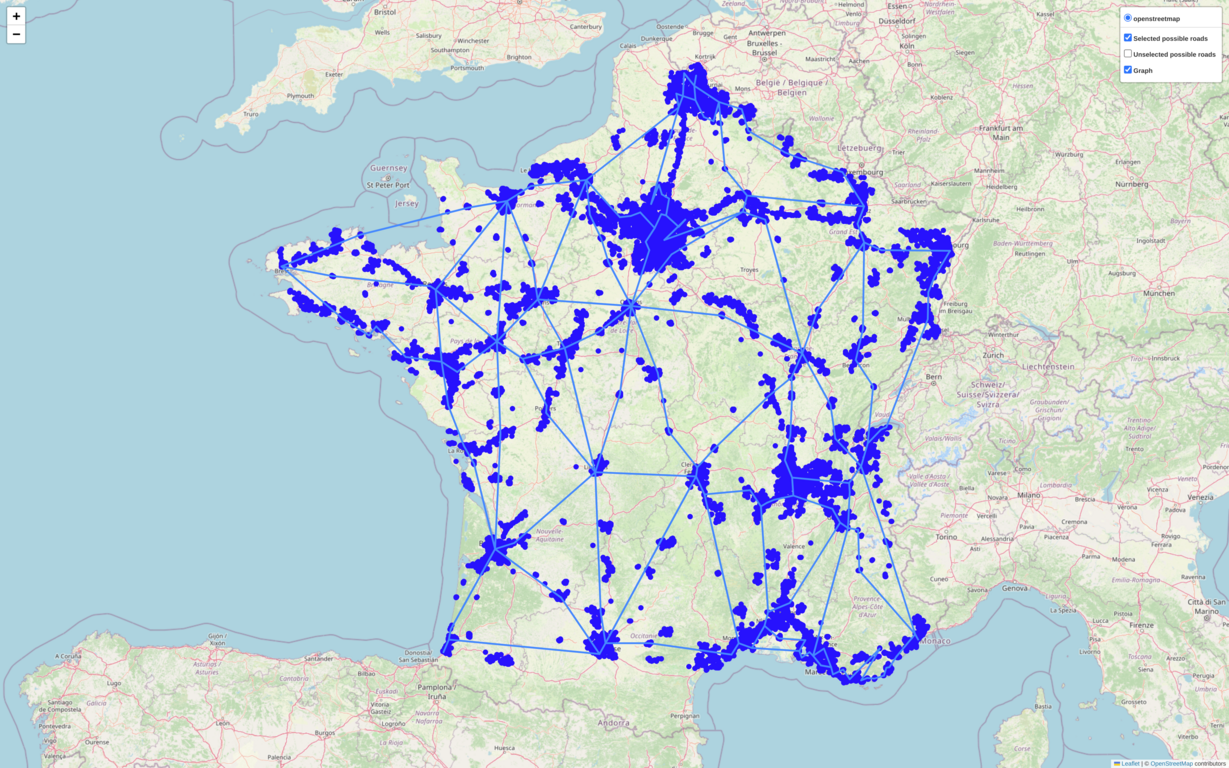
\includegraphics[height=0.6\paperheight]{images/road_detection/roads detected.png}
        \caption{Nodes detected as roads after the method}
    \end{figure}
\end{frame}


\subsection{Further advancement on Coverage Calculation}
\insertsubsectionframe
    
\begin{frame}{Creation of New Database}
    \begin{itemize}
        \item We have created a new database containing detailed information about base stations and their antennas in Normandy, France.
    \end{itemize}
    \begin{block}{Database Fields}
        \begin{itemize}
            \item Station ID (\texttt{id\_station\_anfr})
            \item Latitude and Longitude
            \item Department and Commune Names
            \item Presence of 2G, 3G, 4G, and 5G technologies
            \item Antenna Dimensions and Azimuths
        \end{itemize}
    \end{block}
\end{frame}
    
\begin{frame}{Program for Visualization}
    \begin{itemize}
        \item We implemented a Python program to visualize the base stations on a map and analyze their coverage using Voronoi diagrams.
    \end{itemize}
    \begin{block}{Key Steps in the Program}
        \begin{itemize}
            \item Load and clean the data.
            \item Add markers and pop-ups for each base station.
            \item Calculate and visualize Voronoi cells and antenna sectors.
        \end{itemize}
    \end{block}    
    \begin{block}{Visualization Results}
        \begin{itemize}
            \item The map is centered on Normandy and shows base stations as markers.
            \item Each marker provides detailed information about the station and its antennas.
            \item Voronoi tessellation is used to visualize the coverage area of each base station.
            \item Antenna azimuths are displayed to indicate coverage directions.
        \end{itemize}
    \end{block}
\end{frame}

\begin{frame}
    \frametitle{Example Visualization}
    \begin{center}
        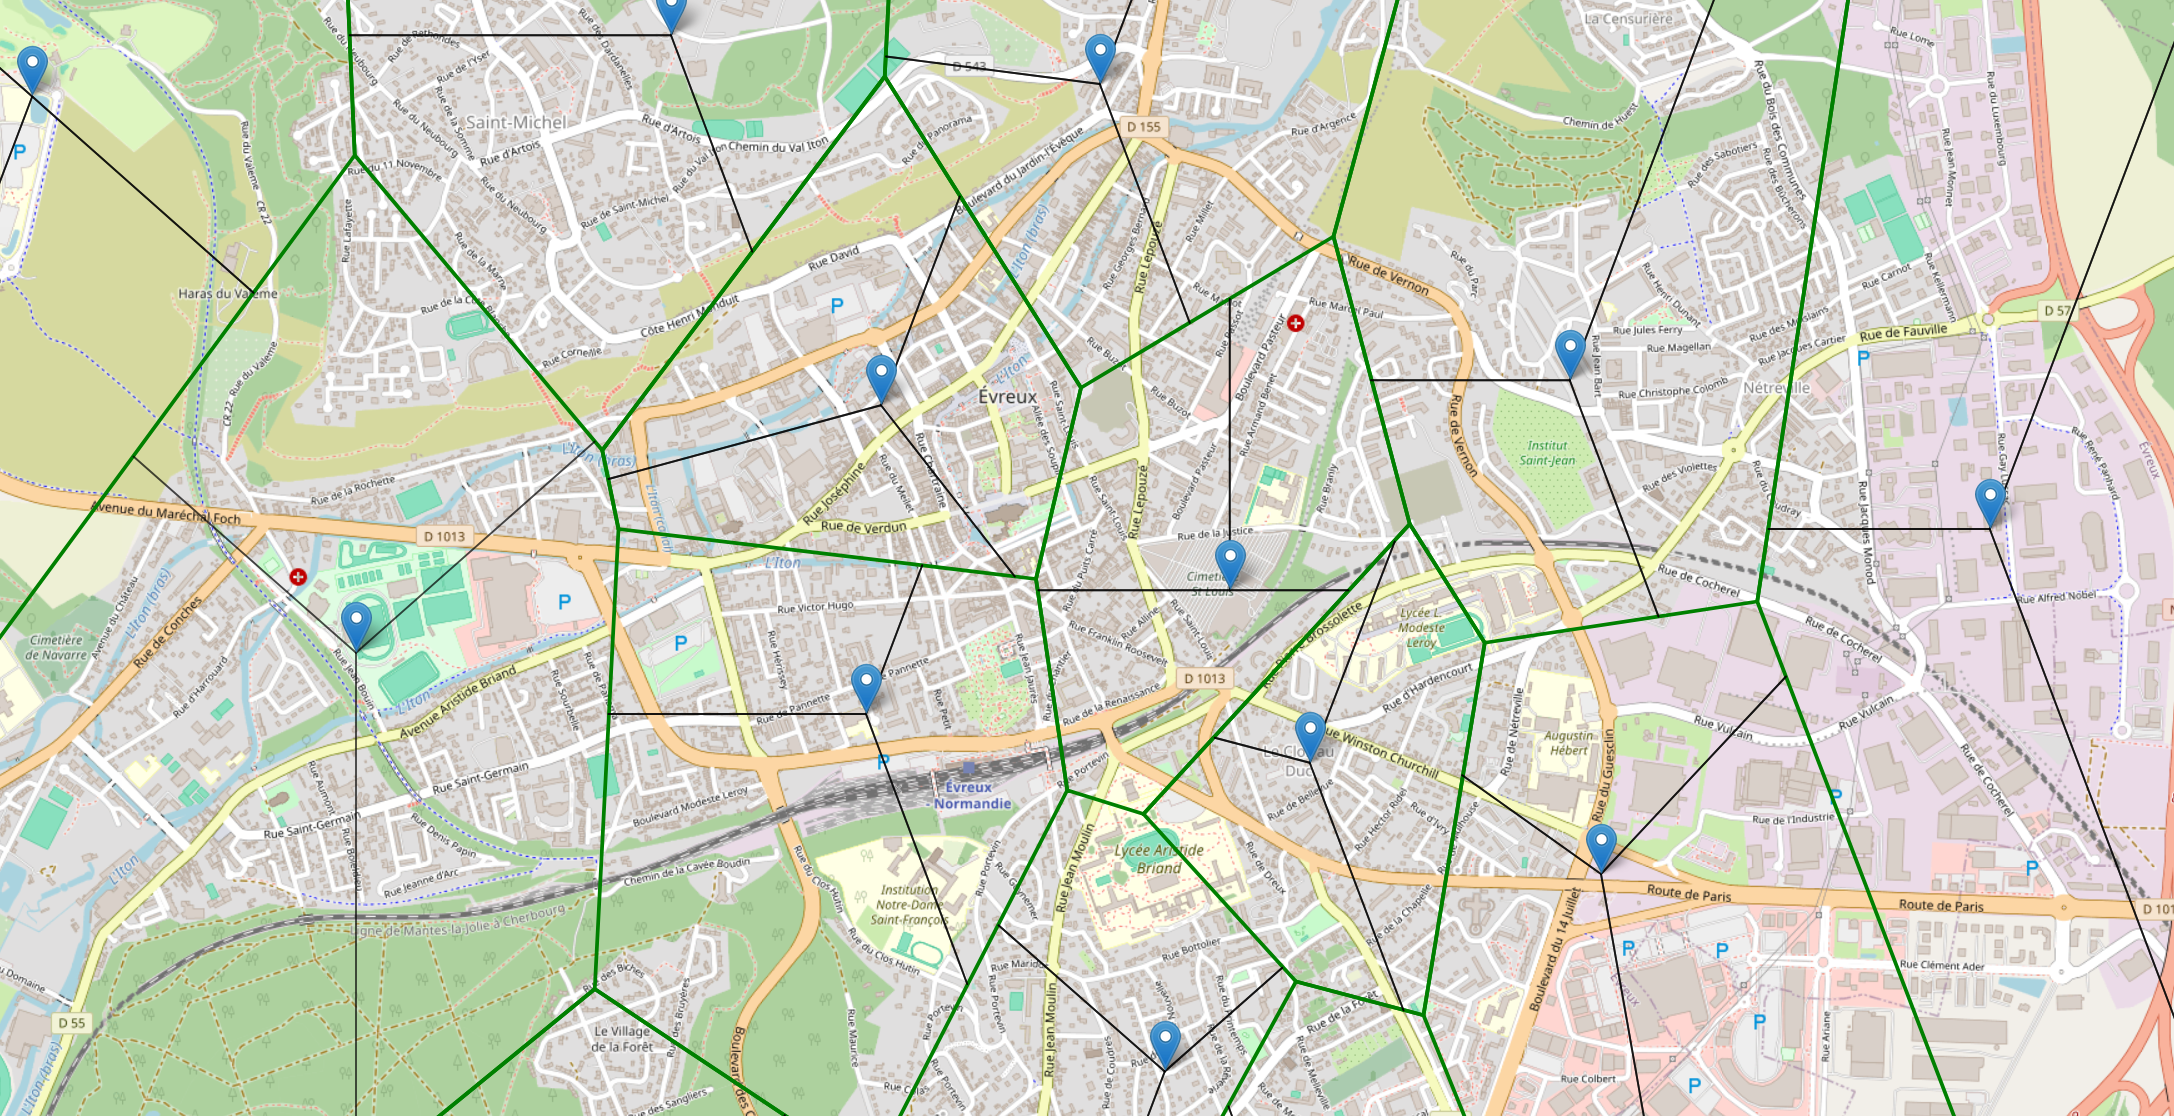
\includegraphics[width=0.5\textwidth]{images/Altair/antenn-vizualization.png}
    \end{center}
    \begin{itemize}
        \item The green lines represent Voronoi boundaries.
        \item The markers indicate base station locations with detailed popup information.
        \item Direction lines show the azimuths of the antennas.
    \end{itemize}
\end{frame}

